\documentclass[12pt]{article}
\usepackage[utf8]{inputenc}
\usepackage[T2A]{fontenc}
\usepackage[russian]{babel}
\usepackage{amsmath}
\usepackage{amssymb}
\usepackage{dsfont}
\usepackage[dvipsnames]{xcolor}
\usepackage{setspace}
\usepackage{multirow}
\usepackage[a4paper, outer=1.5cm, inner=1.5cm, top=1cm, bottom=1cm]{geometry}
\usepackage{graphicx}
\usepackage{skull}
\usepackage{wasysym}
\usepackage{float}
\graphicspath{{.images/}}
\usepackage{hyperref}
\hypersetup{colorlinks=true, linkcolor=blue, filecolor=magenta, urlcolor=cyan}
\usepackage[firstpage]{draftwatermark}
\SetWatermarkText{
    $\qquad\qquad\qquad\qquad\qquad$\parbox{7cm}{\begin{center}
    
\includegraphics[width = 0.08\textwidth]{lion-logo.png}\bigskip\\~\bigskip\\~\vspace{-24mm}\\~\end{center}}
}
\SetWatermarkAngle{0}
\SetWatermarkScale{1.5}
\usepackage{etoolbox}

\newtoggle{ifsolved}
\newtoggle{needhelp}
\newcounter{num}
\setcounter{num}{1}

\newcommand{\newnum}{\par\textbf{\textnumero\arabic{num}}\stepcounter{num}}
\newcommand{\sol}{\vspace{3mm}\par\textbf{Решение: }}
\newcommand{\ans}{\vspace{3mm}\par\textbf{Ответ: }}
\newcommand{\hint}{\vspace{3mm}\par\textbf{Подсказка: }}
\newcommand{\mode}[1]{
\ifstrequal{#1}{0}{\togglefalse{ifsolved}\togglefalse{needhelp}}{\ifstrequal{#1}{1}{\togglefalse{ifsolved}\toggletrue{needhelp}}{\ifstrequal{#1}{2}{\toggletrue{ifsolved}\togglefalse{needhelp}}{\toggletrue{ifsolved}\toggletrue{needhelp}}}}} %if 0 - if 1 - if 2 - else
%\newenvironment{problem}[8]{%#1, #2, #3
%\parbox{\linewidth}{\vspace{4mm}\ifstrequal{#4}{(лёгкая)}{\newnum\textbf{.}}{\newnum\textbf{*.} } \\ #5}
%\iftoggle{ifsolved}{\sol #6}{}
%\iftoggle{ifsolved}{\ans #7}{}
%\iftoggle{needhelp}{\hint #8}{}}

\newenvironment{problem}[8]{%#1, #2, #3
\parbox{\linewidth}{\vspace{5mm}\ifstrequal{#4}{(лёгкая)}{\newnum\textbf{.}}{\newnum\textbf{*.} } \\ #5}
\iftoggle{ifsolved}{\sol #6}{}

\iftoggle{ifsolved}{\parbox{\linewidth}{\ans #7}}{}
\iftoggle{needhelp}{\parbox{\linewidth}{\hint #8}}{}}

\newenvironment{mylist} %custom list
{ \begin{itemize}
    \setlength{\itemsep}{0pt}
    \setlength{\parskip}{0pt}
    \setlength{\parsep}{0pt}     }
{ \end{itemize}                  }

\newenvironment{homeass}[1]{\vspace*{-1.5cm}
\iftoggle{ifsolved}{
    \section*{\center{Решение домашнего задания к #1.}}
}{
    \section*{\center{\textcolor{Sepia}{Домашнее задание к #1}}}
} \vspace{7mm}\large}

\parindent=0pt
\pagestyle{empty}
%$\!$[\arabic{class}.\arabic{num}]
%\ifnumcomp{\value{counter}}{>}{1}{true}{false}
%\definecolor{Gray}{gray}{0.9}
%\definecolor{mypink}{RGB}{219, 48, 122}
%\newcolumntype{g}{>{\columncolor{Gray}}p{2.8cm}}

\begin{document}
\large
\mode{7}
%0 for problems without hints
%1 for problems + hints
%2 for problems + solutions + answers
%else: show all

{\centering\section*{СПИСОК ЗАДАЧ}}

{\centering\subsection*{\smallskip\\\textcolor{green}{\textbf{Полезные вещи, которые можно и нужно копипастить:}}}}

\subsection*{\textcolor{Emerald}{\textbf{Полезные шпаргалки по LaTeXу:}}}

\textbf{Пример вставки рисунка:}

\begin{minipage}{\linewidth}
    \begin{minipage}{0.54\linewidth}
    см. рисунок справа\\
    Текст к собственно пикче, примерно всегда это либо развёрнутое описание, либо большая часть решения задачи --- стремимся экономить пространство, если это можно сделать.
    \end{minipage}
    \hspace{0.05\linewidth}
    \begin{minipage}{0.4\linewidth}
    \begin{figure}[H] 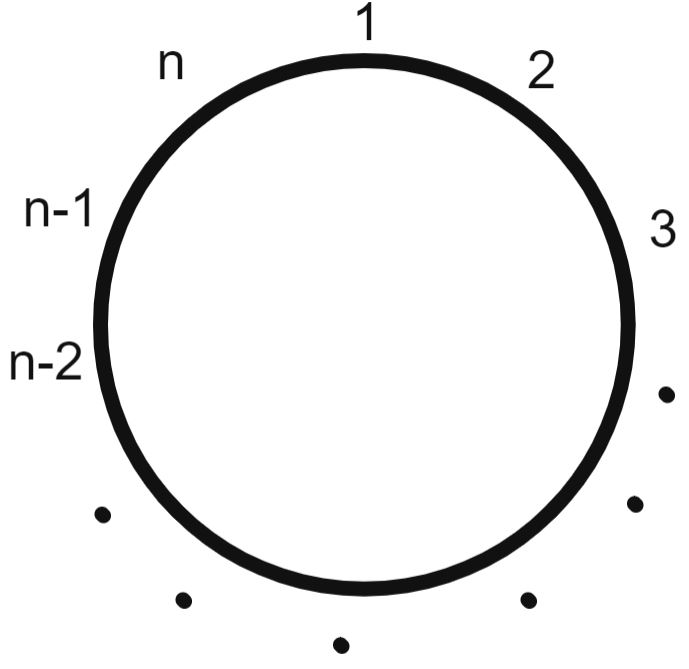
\includegraphics[width=\linewidth]{sol3} %тут поменять имя пикчи
    \end{figure}
    \end{minipage}
\end{minipage}

\textbf{Дефолтные математические знаки и символы:}\\
$\geqslant$,
$\leqslant$,
$a^{b}$,
$x_{i}$,
$\sqrt{a}$,
$\frac{a}{b}$,
$\displaystyle \frac{a}{b}$,
$\cdot$
$\;\Rightarrow\;$,
$\;\Leftrightarrow\;$,
$1{,}2$.
О промежутках:
$a\!b$,
$a\,b$,
$a\:b$,
$a\;b$,
$a\quad b$.

\textbf{Стандартные система и совокупность уравнений / неравенств:}\\
$\left\{
\begin{aligned}
f(x) &= 0 \\
g(x) &= 1
\end{aligned}\right.$

$\left[\begin{aligned}
&\left\{\begin{aligned}
f(x) &\geqslant a \\
g(x) &= b
\end{aligned}\right.\\
&\left\{\begin{aligned}
f(x) &< a \\
g(x) &= -b
\end{aligned}\right.
\end{aligned}\right.$

\subsection*{\textcolor{Emerald}{\textbf{Не математическое, но полезное:}}}
% комментарий в любом месте документа, который нигде не будет видно. Можно использовать для написания заметок-вопросов по задачам
\textbf{Пример таблицы:}

\begin{tabular}{|c|c|c|}
\hline
    $a$ & $b$ & текст
\\\hline
    $c$ & $d$ & мораль
\\\hline
\end{tabular}\\

\textbf{Отступы:} между\smallskip\\ строками\medskip\\ \textbf{Тире} --- это три дефиса.\\
\textbf{Списки:}
\begin{mylist}
\item [$\bullet$] это был пункт а
\item [2)] а это уже пункт номер 2 с изменённым заголовком
\end{mylist}

\subsection*{\textcolor{Emerald}{\textbf{Всё, неупомянутое выше (или если просто что-то не так):}}}
\begin{mylist}
\item [$\bullet$] Решение отдельных вопросов касательно ТеХа нужно искать в \href{https://www.mccme.ru/free-books/llang/newllang.pdf}{Львовском}.

\item [$\bullet$] Найти произвольный символ, который нужен, можно в \href{http://detexify.kirelabs.org/classify.html}{Detexify}.

\item [$\bullet$] Если возникли сомнения при решении, ответ практически ко всем задачам можно проверить с помощью \href{https://www.wolframalpha.com/}{WolframAlpha}.

\item [$\bullet$] Если в задаче нужно создать картинку, то лучше пока отложить эту задачу. Все графики планируется централизованно нарисовать (или перерисовать) в геогебре.

\item [\textcolor{brown}{\textbf{!!}}] Важно ставить \textcolor{red}{\textbf{$\spadesuit$}}
(или просто red) в тело задачи в случае серьёзных вопросов к решению и какой-то вопиющей лажи.

\item [\textcolor{brown}{\textbf{!!}}] Важно ставить \textcolor{olive}{\textbf{$\spadesuit$}}
(или просто olive) в тело задачи в случае не самого удачного текста и кривых отступов.
\end{mylist}

\subsection*{\textcolor{Violet}{\textbf{Комментарии:}}}% а также невидимые комментарии - так можно оставлять заметки-вопросы прямо в задаче, чтобы потом было понятно, в чём вопрос.
\begin{mylist}
\item [$\skull$] Переставлять задачи местами --- очень плохая идея.

\item [$\smiley$] При двойном клике по тексту pdf справа происходит автоматический переход к этому месту в латех-коде, а для обратного перехода можно нажать стрелку вправо (висит сверху между pdf и латех-кодом).

\item [$\smiley$] Если есть размышления, дописывать red/olive к задаче или не дописывать, то лучше всё-таки дописать.

\item [$\skull$] Самое плохое, что можно сделать --- написать в любое поле из трёх (НаписанноеРешение/ВерныйОтвет/Подсказка) только половину того, что надо, никак это не отметить, и потом пойти дальше.\\ Нужно в этот момент писать red/olive в случайном месте задачи, чтобы потом вычислить это с помощью Ctrl+F по всему документу (и это то, что потом будет делаться долго и тщательно)
\end{mylist}

\newpage
\setcounter{num}{1747}

\hypertarget{11.3}{{\centering\section*{\bigskip\\\textcolor{Blue}{\hyperlink{start2}{\textcolor{Blue}{11.3}} Первообразная и интегрирование.}\vspace{-5mm}}}}

\begin{problem}{Правила поиска первообразной.}{11.3.2}{10A}{(лёгкая)}
{Показать, что $F(x) = x\ln x - x + 24e$ является одной из первообразных для функции $f(x) = \ln x$ при $x > 0$.}
{По определению, первообразная функции $f(x)$~--- такая функция $F(x)$, что $F'(x) = f(x)$. Поэтому вычислим производную функции $F(x)$.\\ $F'(x) = \left(x\ln x - x + 24e\right)'$. $24e$~--- какое-то число, на производную оно не влияет $\Rightarrow\; \left(x\ln x - x + 24e\right)' = \ln x + x \cdot \frac1x - 1 + 0 = \ln x$. На указанном интервале логарифм всюду определен, разрывов у $f$ нет. Доказано!}
{$F'(x) = f(x) = \ln x$, при $x > 0$ это непрерывная функция.}{Надо взять производную от функции $F(x)$.}
\end{problem}

\begin{problem}{Правила поиска первообразной.}{11.3.2}{10A}{(лёгкая)}
{Показать, что $F(x) = 3 + \tg\frac{x}{2}$ является первообразной для функции \\$\displaystyle f(x) = \frac{1}{2\cos^2\frac{x}{2}}$ на интервале $(-\pi; \pi)$.}
{По определению, первообразная функции $f(x)$~--- такая функция $F(x)$, что $F'(x) = f(x)$. Поэтому вычислим производную функции $F(x)$.\\ $F'(x) = \left(3 + \tg\frac{x}{2}\right)' = \left(\tg\frac{x}{2}\right)' = \frac{1}{\cos^2 \frac{x}{2}} \cdot \frac12 = \frac{1}{2\cos^2 \frac{x}{2}}$. На указанном интервале $\cos \frac x2$ не обращается в 0, функция определена и всюду непрерывна. Доказано!}
{$F'(x) = f(x) = \frac{1}{2\cos^2 \frac{x}{2}}$, на интервале $(-\pi; \pi)$ это непрерывная функция.}{Надо взять производную от функции $F(x)$.}
\end{problem}

\begin{problem}{Правила поиска первообразной.}{11.3.2}{10A}{*}
{Показать, что функция $F(x) = \ln|x| + \ln|x - 1|$ является первообразной для функции $\displaystyle f(x) = \frac{2x - 1}{x^2 - x}$.}
{По определению, первообразная функции $f(x)$~--- такая функция $F(x)$, что $F'(x) = f(x)$. Поэтому вычислим производную функции $F(x)$. Отдельно рассмотрим интервалы $(-\infty; 0)$, $(0; 1)$, $(1; +\infty)$. На первом интервале $F'(x) = \left(\ln(-x) + \ln(1 - x)\right)' = \frac{1}{-x}\cdot(-1) + \frac{1}{1 - x} \cdot (-1) = \frac1x + \frac{1}{x - 1} = \frac{2x - 1}{x^2 - x}$. На втором интервале $F'(x) = \left(\ln x + \ln(1 - x)\right)' = \frac{1}{x} + \frac{1}{1 - x} \cdot (-1) = \frac1x + \frac{1}{x - 1} = \frac{2x - 1}{x^2 - x}$. \\ Наконец, на интервале $(1; +\infty)$ имеем $F'(x) = \left(\ln x + \ln(x - 1)\right)' = \frac1x + \frac{1}{x - 1} = \frac{2x - 1}{x^2 - x}$.\\ На $R\backslash\{0; 1\}$ $f(x)$ определена, разрывов там нет. Доказано!}
{$F'(x) = f(x)$ (в ООФ $f(x)$, на $R\backslash\{0; 1\}$).}{Надо взять производную от функции $F(x)$, рассмотрев все случаи.}
\end{problem}

\begin{problem}{Правила поиска первообразной.}{11.3.2}{10A}{(лёгкая)}
{Показать, что $F(x) = \frac{x^2}{2} - x - \ln|x + 1| + 5$ является одной из первообразных для функции $\displaystyle f(x) = \frac{x^2 - 2}{x + 1}$.}
{НаписанноеРешение}
{ВерныйОтвет}{Подсказка}
\end{problem}

\begin{problem}{Правила поиска первообразной.}{11.3.2}{10A}{(лёгкая)}
{Найти какую-нибудь первообразную для функции $y = \cos x - 4x$.}
{Как нам известно, $(\sin x)' = \cos x$, $(x^2)' = 2x$.\\ Поэтому функция $F(x) = \sin x - 2x^2$ будет первообразной для  $y$.\\ Проверка: $F'(x) = (\sin x - 2x^2)' = (\sin x)' - 2(x^2)' = \cos x - 4x = y$.}
{Например, $F(x) = \sin x - 2x^2$.}{$F'(x) = y$.}
\end{problem}

\begin{problem}{Правила поиска первообразной.}{11.3.2}{10A}{(лёгкая)}
{Найти общий вид первообразных для функции $y = 8x^3 + 4x + 1$.}
{Согласно таблице первообразных, первообразной для функции $x^n$ \\является функция $\frac{1}{n + 1}x^{n + 1}$. В силу линейности получаем $8\cdot \frac14x^4 + 4\cdot\frac12x^2 + x + C = 2x^4 + 2x^2 + x + C$. Это и есть общий вид первообразной~--- выбрать конкретную первообразную можно, зафиксировав константу $C$ (задав начальное условие).}
{$F(x) = 2x^4 + 2x^2 + x + C$~--- общий вид первообразной функции $y$.}{Использовать таблицу первообразных и линейность первообразной.}
\end{problem}

\begin{problem}{Правила поиска первообразной.}{11.3.2}{10A}{(лёгкая)}
{Найти первообразную для функции $\displaystyle y = \frac{2}{3 - x}$.}
{НаписанноеРешение}
{ВерныйОтвет}{Подсказка}
\end{problem}

\begin{problem}{Правила поиска первообразной.}{11.3.2}{10A}{(лёгкая)}
{Найти первообразную для функции $\displaystyle y = \frac{4}{x + 1}$.}
{Согласно таблице первообразных, нам известна первообразная функции $\frac 1x$: она равна $\ln |x| + C$ (не забываем модуль и константу!). Используем тот факт, что $\frac{1}{k}F(kx + b)$~--- первообразная для $f(kx + b)$ тогда и только тогда, когда $F(x)$~--- первообразная для $f(x)$. В силу этого и линейности получаем, что первообразной для функции $y = \frac{4}{x + 1}$ будет функция $F(x) = 4\ln|x + 1| + C$.}
{$F(x) = 4\ln|x + 1| + C$.}{Не забудь модуль; используй факт о первообразной для $f(kx + b)$.}
\end{problem}

\begin{problem}{Правила поиска первообразной.}{11.3.2}{10A}{(лёгкая)}
{Найти первообразную для функции $\displaystyle y = 3e^{\frac{3}{4}x}$.}
{Табличной первообразной для функции $f(x) = e^x$ является функция $F(x) = e^x + C$. $y = 3e^{\frac34 x} = 3f(\frac34 x)$, поэтому её первообразная равна $3\cdot\frac{1}{\frac34}F(\frac34x) = 4F(\frac34x) = 4e^{\frac{3}{4}x} + C$.}
{Первообразной для $y$ является функция $4e^{\frac{3}{4}x} + C$.}{Используй линейность и факт о первообразной для $f(kx + b)$.}
\end{problem}

\begin{problem}{Правила поиска первообразной.}{11.3.2}{10A}{*}
{Найти первообразную для функции $\displaystyle f(x) = \frac{x}{x - 1}$.}
{Данная функция не является табличной. Используем хитрый трюк: $f(x) = \frac{x}{x - 1} = \frac{x - 1 + 1}{x - 1} = 1 + \frac{1}{x - 1}$. Теперь в силу линейности интегрирования нетрудно заметить, что $F(x) = x + \ln|x - 1| + C$. Это и есть первообразная функции $f$.}
{$F(x) = x + \ln|x - 1| + C$.}{Представь дробь в виде суммы двух простейших дробей.}
\end{problem}

\begin{problem}{Правила поиска первообразной.}{11.3.2}{10A}{*}
{Найти первообразную для функции $\displaystyle f(x) = \frac{2}{x^2 - 1}$.}
{НаписанноеРешение}
{ВерныйОтвет}{Подсказка}
\end{problem}

\begin{problem}{Правила поиска первообразной.}{11.3.2}{10A}{*}
{Найти первообразную для функции $\displaystyle f(x) = \frac{5x - 1}{x^2 - x - 2}$.}
{Данная функция $f(x)$ не является табличной.\\ Отметим, что $x^2 - x - 2 = (x + 1)(x - 2)$, а значит, данную дробь можно представить в виде суммы двух простейших дробей: $\frac{5x - 1}{x^2 - x - 2} = \frac{5x - 1}{(x + 1)(x - 2)} = \frac{A}{x + 1} + \frac{B}{x - 2}$, где $A$ и $B$~--- какие-то коэффициенты (обычный метод неопределённых коэффициентов).\smallskip\\ То есть $A(x - 2) + B(x + 1) = 5x - 1$. Отсюда получаем систему уравнений: $\left\{\begin{aligned}
A + B &= 5\\
-2A + B &= -1
\end{aligned}\right. \;\Rightarrow\; \left\{\begin{aligned}
A &= 2\\
B &= 3.
\end{aligned}\right.\quad$ То есть $\displaystyle f(x) = \frac{5x - 1}{x^2 - x - 2} = \frac{2}{x + 1} + \frac{3}{x - 2}$.\smallskip\\ Эту функцию мы уже можем интегрировать (первообразная для $\frac1x$ равна $\ln|x|$), в итоге получаем $F(x) = 2\ln|x + 1| + 3\ln|x - 2| + C$.}
{Первообразная для функции $f(x)$ равна $2\ln|x + 1| + 3\ln|x - 2| + C$.}{Представь дробь в виде суммы двух простейших дробей.}
\end{problem}

\begin{problem}{Правила поиска первообразной.}{11.3.2}{10A}{*}
{Найти первообразную для функции $f(x) = \cos^2 x$.}
{НаписанноеРешение}
{ВерныйОтвет}{Подсказка}
\end{problem}

\begin{problem}{Правила поиска первообразной.}{11.3.2}{10A}{*}
{Найти первообразную для функции $f(x) = \sin^2 x$.}
{Данной функции нет в таблице простейших производных. Однако, можно воспользоваться хитрым приёмом. Вспомним формулу понижения степени: $\cos 2x = 1 - 2\sin^2 x \;\Rightarrow\; f(x) = \sin^2 x = \frac12(1 - \cos 2x)$.\\ То есть, можно найти первообразную для $\frac12 - \frac12\cos2x$, а эта задача гораздо проще: поскольку $F(kx + b)$~--- первообразная для $\frac1k f(kx + b)$, получаем, что первообразной для функции $f(x) = \sin^2x = \frac12 - \frac12\cos2x$ является $F(x) = \frac x2 - \frac14\sin 2x + C$.}
{Первообразная имеет вид $F(x) = \frac x2 - \frac14\sin 2x + C$.\\
На случай, если есть возмущения в духе <<так же нельзя делать>>, вот проверка: $F(x) = \frac x2 - \frac14\sin 2x + C = \frac x2 - \frac12\sin x\cos x + C \;\Rightarrow\; F'(x) = \frac12 - \frac12 (\sin x \cos x)' = \frac12 - \frac12((\sin x)'\cos x + \sin x (\cos x)') = \frac12 - \frac12 \cos^2 x + \frac12 \sin^2x = \frac12(1 - \cos^2 x) + \frac12\sin^2 x = \frac12\sin^2 x + \frac12\sin^2 x = \sin^2x = f(x)$.}{Формула понижения степени для тригонометрических функций.}
\end{problem}

\begin{problem}{Правила поиска первообразной.}{11.3.2}{10A}{*}
{Дана функция $f(x) = |x|$. Найти её первообразную.}
{Рассмотрим функцию $f(x)$ отдельно для неотрицательных и отрицательных $x$. Для отрицательных $f(x) = -x$, и $F(x) = -\frac{x^2}{2}$. Для неотрицательных $f(x) = x$, и $F(x) = \frac{x^2}{2}$. Таким образом, $F(x) = \left\{\begin{aligned}
-\frac{x^2}{2} + C, \text{ если } x < 0\\
\frac{x^2}{2} + C, \text{ если } x \geqslant 0
\end{aligned}\right. =$ \\ $\displaystyle = \frac12\text{sgn}(x)\cdot x^2 + C$, где $\text{sgn}(x)$~--- функция, возвращающая знак числа.}
{$F(x) = \frac12\text{sgn}(x)\cdot x^2 + C$.}{Рассмотреть отдельно два случая~--- для отрицательных $x$ и для неотрицательных. Нужно не забыть константу, а также убедиться, что функция $F(x)$ непрерывна в 0.}
\end{problem}

\begin{problem}{Правила поиска первообразной.}{11.3.2}{10A}{(лёгкая)}
{Найти первообразную для функции $y = 2x + 1$, если известно, что график этой первообразной проходит через начало координат.}
{Согласно таблице первообразных, первообразная функции $y$ имеет вид $F(x) = x^2 + x + C$. Найдём $C$, учитывая заданные ограничения~--- раз $F(x)$ проходит через начало координат, $F(0) = 0$, откуда $F(0) = C = 0 \;\Rightarrow\; F(x) = x^2 + x$.}
{Первообразная для функции $y = 2x + 1$, которая проходит через начало координат~--- функция $F(x) = x^2 + x$.}{Условие задаёт константу.}
\end{problem}

\begin{problem}{Правила поиска первообразной.}{11.3.2}{10A}{(лёгкая)}
{Найти функцию $F(x)$, если известно, что $F'(x) = 4x^3 - 3x^2$, и $F(1) = 3$.}
{НаписанноеРешение}
{ВерныйОтвет}{Подсказка}
\end{problem}

\begin{problem}{Правила поиска первообразной.}{11.3.2}{10A}{(лёгкая)}
{Найти функцию $F(x)$, график которой проходит через точку $M$, если известно, что $F'(x) = 4x^2 + 9x^{-2}$, а $M = (3; -2)$.}
{Используя таблицу первообразных, имеем первообразную $\frac{1}{n + 1}x^{n + 1}$ для $x^n$, откуда (в силу линейности первообразной) получаем её общий вид:\\ $F(x) = 4\cdot\frac13x^3 + 9\cdot\frac{1}{-1}x^{-1} + C = \frac{4}{3}x^3 - \frac{9}{x} + C$. Находим $C$: раз график $F(x)$ проходит через точку $M$, $F(3) = -2 \;\Rightarrow\; \frac43\cdot3^3 - \frac93 + C = 36 - 3 + C = -2 \;\Rightarrow\; C = -35$.\smallskip\\
Таким образом, $F(x) = \frac{4}{3}x^3 - \frac{9}{x} - 35$.}
{Искомая функция имеет вид $F(x) = \frac{4}{3}x^3 - \frac{9}{x} - 35$.}{Константа находится с помощью уравнения $F(3) = -2$.}
\end{problem}

\begin{problem}{Правила поиска первообразной.}{11.3.2}{10A}{(лёгкая)}
{Найти функцию $F(x)$, график которой проходит через точку $M$, если известно, что $F'(x) = \sin 2x$, а $M = (0; 1)$.}
{Функция $\sin x$ имеет табличную первообразную $-\cos x + C$ (поскольку $(-\cos x + C)' = \sin x$). Используя это, а также то, что $\frac1kF(kx + b)$~--- первообразная для $f(kx + b)$, получаем, что $F(x) = -\frac12\cos 2x + C$. График функции $F(x)$ проходит через точку $(0; 1)$, а значит, $F(0) = 1$, откуда $-\frac12\cos 0 + C = 1$.\smallskip\\ $\cos 0 = 1 \;\Rightarrow\; C = 1 + \frac12 = \frac32$. Следовательно, $F(x) = -\frac12\cos 2x + \frac32 = \frac{3 - \cos 2x}{2}$.}
{$F(x) = -\frac12\cos 2x + \frac32$.}{Константа находится из условия $F(0) = 1$.}
\end{problem}

\begin{problem}{Неопределённый интеграл.}{11.3.3}{10A}{(лёгкая)}
{Вычислить неопределённый интеграл $\displaystyle \int\limits \!\left(\frac{4}{\cos^2 2x} - 1\right) dx$.}
{НаписанноеРешение}
{ВерныйОтвет}{Подсказка}
\end{problem}

\begin{problem}{Неопределённый интеграл.}{11.3.3}{10A}{(лёгкая)}
{Вычислить неопределённый интеграл $\displaystyle \int\limits \frac{2x + 3}{x^2 - 9} \,dx$.}
{НаписанноеРешение}
{ВерныйОтвет}{Подсказка}
\end{problem}

\begin{problem}{Неопределённый интеграл.}{11.3.3}{10A}{(лёгкая)}
{Вычислить неопределённый интеграл $\displaystyle \int\limits \!\frac{5x}{(x - 1)^3} \,dx$.}
{Разложим данную дробь на простейшие: используем метод неопределённых коэффициентов: $\displaystyle \frac{5x}{(x - 1)^3} = \frac{A}{x-1} + \frac{B}{(x-1)^2} + \frac{C}{(x-1)^3}$. Тогда после приведения к общему знаменателю получаем, что $5x \equiv A(x-1)^2 + B(x-1) + C$.\\
Отсюда $Ax^2 + (B - 2A)x + (A - B + C) \equiv 5x$, и поскольку эти два многочлена должны быть тождественно равны, имеем $A = 0$, $\,B = 5$, $\,C = 5$.\\ То есть, $\displaystyle \frac{5x}{(x - 1)^3} = \frac{5}{(x-1)^2} + \frac{5}{(x-1)^3}$.\\
$\displaystyle \int\limits \!\frac{5x}{(x - 1)^3} \,dx = \int\limits \!\!\left(\frac{5}{(x - 1)^2} + \frac{5}{(x - 1)^3}\!\right) dx = \int\limits \!\frac{5}{(x - 1)^2} \,dx + \int\limits \!\frac{5}{(x - 1)^3} \,dx = 5\cdot\int\limits \!\frac{1}{(x - 1)^2} \,dx + 5\cdot\int\limits \!\frac{1}{(x - 1)^3} \,dx = -\frac{5}{x - 1} -\frac{5}{2(x - 1)^2} + C$.\smallskip\\
Итого, $\displaystyle \int\limits \!\frac{5x}{(x - 1)^3} \,dx = -\frac{5}{x - 1} -\frac{5}{2(x - 1)^2} + C = -\frac{10x - 5}{2(x-1)^2} + C$.}
{$\displaystyle \int\limits \!\frac{5x}{(x - 1)^3} \,dx = -\frac{10x - 5}{2(x-1)^2} + C$.}{Разложи данную дробь на простейшие.}
\end{problem}

\begin{problem}{Неопределённый интеграл.}{11.3.3}{10A}{(лёгкая)}
{Вычислить неопределённый интеграл $\displaystyle \int\limits \!\frac{x^2}{(x - 1)(x - 2)(x - 3)} \,dx$.}
{Данную дробь можно разложить на простейшие:\\ $\displaystyle \frac{x^2}{(x - 1)(x - 2)(x - 3)} = \frac{A}{x - 1} + \frac{B}{x - 2} + \frac{C}{x - 3}$. После приведения к общему знаменателю получаем, что числители дробей тождественно равны: $x^2 \equiv A(x-2)(x-3) + B(x-1)(x-3) + C(x-1)(x-2) = A(x^2 - 5x + 6) + B(x^2 - 4x + 3) + C(x^2 - 3x + 2)$.\\
Это означает, что $A + B + C = 1$, $\,-5A - 4B - 3C = 0$, $\,6A + 3B + 2C = 0$.\smallskip\\ Решаем систему уравнений: $\left\{\begin{aligned}
A + B + C = 1\\
-5A - 4B - 3C = 0\\
6A + 3B + 2C = 0
\end{aligned}\right. \;\Rightarrow\; \left\{\begin{aligned}
A + B + C = 1\\
-A + C = 4\\
4A + B = -2
\end{aligned}\right. \;\Rightarrow$ \\
$\Rightarrow\;\left\{\begin{aligned}
B = -2 - 4A\\
C = 4 + A\\
A - 2 - 4A + 4 + A = 1
\end{aligned}\right. \;\Rightarrow\; \left\{\begin{aligned}
A = 0{,}5\\
B = -4\\
C = 4{,}5
\end{aligned}\right.$\\
Таким образом, $\displaystyle \frac{x^2}{(x - 1)(x - 2)(x - 3)} = \frac{0{,}5}{x - 1} - \frac{4}{x - 2} + \frac{4{,}5}{x - 3}$.\\
Следовательно, $\displaystyle \int\limits \!\frac{x^2}{(x - 1)(x - 2)(x - 3)} \,dx = \displaystyle \int\limits \!\left(\frac{0{,}5}{x - 1} - \frac{4}{x - 2} + \frac{4{,}5}{x - 3}\right) \,dx = 0{,}5\int\limits \!\frac{dx}{x - 1} - 4\int\limits\!\frac{dx}{x - 2} + 4{,}5\int\limits\!\frac{dx}{x - 3} = \tfrac12\ln|x-1| - 4\ln|x-2| + \tfrac92\ln|x-3| + C$.}
{$\displaystyle \int\limits \!\frac{x^2}{(x - 1)(x - 2)(x - 3)} \,dx = \tfrac12\ln|x-1| - 4\ln|x-2| + \tfrac92\ln|x-3| + C$.}{Разложи данную дробь на простейшие.}
\end{problem}

\begin{problem}{Определённый интеграл. Формула Ньютона-Лейбница.}{11.3.4}{10A}{(лёгкая)}
{(Положительность интеграла) Объяснить, почему, если интегрируемая функция $f(x)$ неотрицательна на отрезке $[a, b]$, то $\displaystyle \int\limits_{a}^{b} f(x)\,dx \geqslant 0$.}
{НаписанноеРешение}
{ВерныйОтвет}{Подсказка}
\end{problem}

\begin{problem}{Определённый интеграл. Формула Ньютона-Лейбница.}{11.3.4}{10A}{(лёгкая)}
{(Линейность интеграла) Объяснить, почему для интегрируемых на отрезке $[a, b]$ функций $f(x)$ и $g(x)$ функция $pf(x) + qg(x)$ ($p$, $q$~--- вещественные числа) также интегрируема и $\,\displaystyle \int\limits_{a}^{b} (pf(x) + qg(x))\,dx = p\int\limits_{a}^{b} f(x)\,dx + q\int\limits_{a}^{b} g(x)\,dx$.}
{НаписанноеРешение}
{ВерныйОтвет}{Подсказка}
\end{problem}

\begin{problem}{Определённый интеграл. Формула Ньютона-Лейбница.}{11.3.4}{10A}{(лёгкая)}
{(Аддитивность интеграла) Объяснить, почему $\displaystyle \int\limits_{a}^{b}\! f(x)\,dx\, + \int\limits_{b}^{c} \!f(x)\,dx = \int\limits_{a}^{c} \!f(x)\,dx$.}
{НаписанноеРешение}
{ВерныйОтвет}{Подсказка}
\end{problem}

\begin{problem}{Определённый интеграл. Формула Ньютона-Лейбница.}{11.3.4}{10A}{(лёгкая)}
{Вычислить интеграл от 3 до 6 от функции $f(x) = 2x$.}
{НаписанноеРешение}
{ВерныйОтвет}{Подсказка}
\end{problem}

\begin{problem}{Определённый интеграл. Формула Ньютона-Лейбница.}{11.3.4}{10A}{(лёгкая)}
{Вычислить интеграл от $-1$ до 1 от функции $f(x) = x^{2}$.}
{Для того чтобы вычислить определённый интеграл $\int\limits_{-1}^1 x^2 dx$, найдем первообразную для подынтегральной функции $f(x) = x^2$. Данная функция имеет табличную первообразную $F(x) = \frac13x^3 + C$. Используем результат формулы Ньютона-Лейбница: $\int\limits_{-1}^1 x^2 dx = F(1) - F(-1) = \left.\frac13x^3 \right|_{-1}^1 = \frac13 - (-\frac13) = \frac23$.}
{Интеграл от $-1$ до 1 от функции $f(x) = x^2$ равен $\int\limits_{-1}^1 x^2 dx = \frac23$.}{Найди первообразную и используй формулу Ньютона-Лейбница.}
\end{problem}

\begin{problem}{Определённый интеграл. Формула Ньютона-Лейбница.}{11.3.4}{10A}{(лёгкая)}
{Вычислить определённый интеграл $\displaystyle \int\limits_{-1}^{3}x^3 \,dx$.}
{Для того, чтобы вычислить определённый интеграл, сначала найдём неопределённый интеграл: $\int\limits x^3 \,dx = \frac14 x^4 + C$. По формуле Ньютона-Лейбница получаем $\int\limits_{-1}^{3}x^3 \,dx = F(b) - F(a) = \left.\frac14x^4\right|_{-1}^3 = \frac{81}{4} - \frac14 = \frac{80}{4} = 20$.}
{Определённый интеграл $\int\limits_{-1}^{3}x^3 \,dx$ равен 20.}{Неопределённый интеграл $+$ формула Ньютона-Лейбница.}
\end{problem}

\begin{problem}{Определённый интеграл. Формула Ньютона-Лейбница.}{11.3.4}{10A}{(лёгкая)}
{Вычислить определённый интеграл $\displaystyle \int\limits_{1}^{16}\sqrt[4]{x} \,dx$.}
{НаписанноеРешение}
{ВерныйОтвет}{Подсказка}
\end{problem}

\begin{problem}{Определённый интеграл. Формула Ньютона-Лейбница.}{11.3.4}{10A}{(лёгкая)}
{Вычислить определённый интеграл $\displaystyle \int\limits_{0}^{\pi}\sin x \,dx$.}
{НаписанноеРешение}
{ВерныйОтвет}{Подсказка}
\end{problem}

\begin{problem}{Определённый интеграл. Формула Ньютона-Лейбница.}{11.3.4}{10A}{(лёгкая)}
{Вычислить определённый интеграл $\displaystyle \int\limits_{-2}^{4}(8 + 2x - x^{2}) \,dx$.}
{Для того, чтобы вычислить определённый интеграл, сначала найдём неопределённый интеграл: $\int\limits (8 + 2x - x^{2}) \,dx = 8x + x^2 - \frac13x^3 + C$.\\ По формуле Ньютона-Лейбница получаем $\int\limits_{-2}^{4} (8 + 2x - x^{2}) \,dx = F(4) - F(-2) = \left.(8x + x^2 - \frac13x^3)\right|_{-2}^4 = 8(4 - (-2)) + 4^2 - (-2)^2 -\frac13(4^3 - (-2)^3) = 36$.}
{$\int\limits_{-2}^{4}(8 + 2x - x^{2}) \,dx = 36$. Если нарисовать график, становится видно, что это площадь всего того куска параболы, который находится выше оси абсцисс.}{Неопределённый интеграл $+$ формула Ньютона-Лейбница.}
\end{problem}

\begin{problem}{Определённый интеграл. Формула Ньютона-Лейбница.}{11.3.4}{10A}{*}
{Вычислить определённый интеграл $\displaystyle \int\limits_{1 - e}^{1 - \frac1e} \frac{7 - 3x}{x^2 - 3x + 2} \,dx$.}
{Для того, чтобы вычислить определённый интеграл, нужно сперва вычислить неопределённый. А у нас функция не имеет табличной первообразной.\\ Поэтому разложим данную подынтегральную функцию на простейшие дроби.\vspace{-2mm}
$$x^2 - 3x + 2 = (x - 1)(x - 2) \;\Rightarrow\; \frac{7 - 3x}{x^2 - 3x + 2} = \frac{A}{x - 1} + \frac{B}{x - 2}.$$
\vspace{-6mm}\\
С помощью метода неопределённых коэффициентов находим $A$ и $B$:\\
$A(x - 2) + B(x - 1) = 7 - 3x \;\Rightarrow\; \left\{\begin{aligned}
A + B = -3\\
-2A - B = 7
\end{aligned}\right. \;\Rightarrow\; \left\{\begin{aligned}
A &= -4\\
B &= 1
\end{aligned}\right.$\\
Таким образом, $\displaystyle \frac{7 - 3x}{x^2 - 3x + 2} = \frac{1}{x - 2} - \frac{4}{x - 1}$.\smallskip\\ Первообразной для этой функции является $F(x) = \ln|x - 2| - 4\ln|x - 1| + C$.\smallskip\\
Находим определённый интеграл с помощью формулы Ньютона-Лейбница:\\
$\displaystyle \int\limits_{1 - e}^{1 - \frac1e} \frac{7 - 3x}{x^2 - 3x + 2} \,dx = \int\limits_{1 - e}^{1 - \frac1e} \!\left(\frac{1}{x - 2} - \frac{4}{x - 1}\right) \,dx = \left.\left(\ln|x - 2| - 4\ln|x - 1|\right)\vphantom{\tfrac11}\right|_{1 - e}^{1 - \frac1e} =$\\
$\displaystyle \left(\ln(1 + \tfrac1e) - 4\ln\tfrac1e\right) - \left(\ln(1 + e) - 4\ln e\right) = \ln\left(\frac{e + 1}{e} : (e + 1)\right) + 4 + 4 = 7$.}
{Определённый интеграл $\displaystyle \int\limits_{1 - e}^{1 - \frac1e} \frac{7 - 3x}{x^2 - 3x + 2} \,dx = 7$.}{Разложи дробь в сумму простейших дробей с помощью метода неопределённых коэффициентов.}
\end{problem}

\begin{problem}{Определённый интеграл. Формула Ньютона-Лейбница.}{11.3.4}{10A}{(лёгкая)}
{Вычислить определённый интеграл $\displaystyle \int\limits_{-4}^{4} \sqrt[3]{x} \,dx$.}
{НаписанноеРешение}
{ВерныйОтвет}{Подсказка}
\end{problem}

\begin{problem}{Определённый интеграл. Формула Ньютона-Лейбница.}{11.3.4}{10A}{(лёгкая)}
{Вычислить определённый интеграл $\displaystyle \int\limits_{0}^{2\pi}\cos x \,dx$.}
{Сначала вычислим неопределённый интеграл: $\int\limits\cos x \,dx = \sin x + C$.\\
По формуле Ньютона-Лейбница получаем $\int\limits_{0}^{2\pi}\cos x \,dx = \left.F(x)\right|_{0}^{2\pi} = \sin 2\pi - \sin 0 = 0 - 0 = 0$. Определённый интеграл равен 0.}
{$\int\limits_{0}^{2\pi}\cos x \,dx = 0$.\\ Если нарисовать график, становится понятно, что друг из друга вычитаются площади арок косинусоид, и поскольку они равны по площади, в итоге выходит 0.}{Неопределённый интеграл $+$ формула Ньютона-Лейбница.}
\end{problem}

\begin{problem}{Определённый интеграл. Формула Ньютона-Лейбница.}{11.3.4}{10A}{*}
{Вычислить определённый интеграл $\displaystyle \int\limits_{-5}^{5} \sqrt[3]{x}\cos(\pi x) \,dx$.}
{НаписанноеРешение}
{ВерныйОтвет}{Подсказка}
\end{problem}

\begin{problem}{Определённый интеграл. Формула Ньютона-Лейбница.}{11.3.4}{10A}{*}
{Вычислить определённый интеграл $\displaystyle \int\limits_{-1}^{1} \frac{x^2 + e}{\ctg x} \,dx$.}
{Для начала отметим, что подынтегральная функция $\frac{x^2 + e}{\ctg x} = (x^2 + e)\tg x$ на указанном отрезке непрерывна, в силу чего интеграл существует. Функция $x^2 + e$ является чётной, функция $\tg x = \frac{\sin x}{\cos x}$ является нечётной ($\tg (-x) = \frac{\sin (-x)}{\cos (-x)} = \frac{-\sin x}{\cos x} = -\tg x$). Произведение чётной и нечётной функций является нечётной функцией. Это означает, что график подынтегральной функции $f(x) = \frac{x^2 + e}{\ctg x}$ центрально симметричен относительно начала координат. Но в нашем случае интеграл берётся по симметричному относительно 0 отрезку! Это означает, что\\$\displaystyle \int\limits_{-1}^{1} \frac{x^2 + e}{\ctg x} \,dx = \int\limits_{-1}^{0} \frac{x^2 + e}{\ctg x} \,dx + \int\limits_{0}^{1} \frac{x^2 + e}{\ctg x} \,dx = -\int\limits_{0}^{1} \frac{x^2 + e}{\ctg x} \,dx + \int\limits_{0}^{1} \frac{x^2 + e}{\ctg x} \,dx = 0$.}
{$\displaystyle \int\limits_{-1}^{1} \frac{x^2 + e}{\ctg x} \,dx = 0$ в силу нечётности подынтегральной функции.}{В данной задаче симметрична не только область интегрирования, но и сама подынтегральная функция!}
\end{problem}

\begin{problem}{Определённый интеграл. Формула Ньютона-Лейбница.}{11.3.4}{10A}{*}
{Вычислить определённый интеграл $\displaystyle \int\limits_{(\sqrt{3} - 2)^{-1}}^{2 + \sqrt{3}} \!\!\!\!\!x e^{-\frac{x^2}{2}} \,dx$.}
{Подынтегральная функция не выглядит как табличная первообразная. Попробуем что-нибудь придумать. Для начала, разберёмся со странным нижним пределом интегрирования: $(\sqrt{3} - 2)^{-1} = \frac{1}{\sqrt{3} - 2} = \frac{\sqrt{3} + 2}{3 - 2^2} = -(2 + \sqrt{3})$.\\ Это означает, что интегрирование ведётся по области, симметричной относительно 0. Теперь уже несложно заметить, что подынтегральная функция нечётна: $f(-x) = (-x)e^{-\frac{(-x)^2}{2}} = -xe^{-\frac{x^2}{2}} = -f(x)$. Значит, график подынтегральной функции $f(x)$ центрально симметричен относительно нуля и мы получаем, что\\
$\displaystyle \int\limits_{-(2 + \sqrt{3})}^{2 + \sqrt{3}} \!\!\!\!\!\!x e^{-\frac{x^2}{2}} \,dx\; = \!\!\!\!\int\limits_{-(2 + \sqrt{3})}^{0} \!\!\!\!\!\!x e^{-\frac{x^2}{2}} \,dx\, + \!\!\int\limits_{0}^{2 + \sqrt{3}} \!\!\!x e^{-\frac{x^2}{2}} \,dx = -\!\!\!\!\int\limits_{0}^{2 + \sqrt{3}} \!\!\!x e^{-\frac{x^2}{2}} \,dx\, + \!\!\int\limits_{0}^{2 + \sqrt{3}} \!\!\!x e^{-\frac{x^2}{2}} \,dx = 0$.}
{Определённый интеграл $\displaystyle \int\limits_{(\sqrt{3} - 2)^{-1}}^{2 + \sqrt{3}} \!\!\!\!\!x e^{-\frac{x^2}{2}} \,dx = 0$ в силу нечётности подынтегральной функции и симметричности отрезка интегрирования относительно 0.}{В этой задаче есть целых две симметрии. Найти обе.}
\end{problem}

\begin{problem}{Определённый интеграл. Формула Ньютона-Лейбница. red несобственный}{11.3.4}{10A}{*}
{Определить, сходится или расходится несобственный интеграл $\displaystyle \int\limits_{1}^{+\infty} \frac{1}{x} \, dx$.}
{НаписанноеРешение}
{ВерныйОтвет}{Подсказка}
\end{problem}

\begin{problem}{Определённый интеграл. Формула Ньютона-Лейбница. red несобственный}{11.3.4}{10A}{*}
{Определить, сходится или расходится несобственный интеграл $\displaystyle \int\limits_{1}^{+\infty} \frac{1}{x^2} \, dx$.}
{НаписанноеРешение}
{ВерныйОтвет}{Подсказка}
\end{problem}

\begin{problem}{Определённый интеграл. Формула Ньютона-Лейбница. red несобственный}{11.3.4}{10A}{*}
{Определить, сходится или расходится несобственный интеграл $\displaystyle \int\limits_{-\infty}^{5} \sin x \, dx$.}
{НаписанноеРешение}
{ВерныйОтвет}{Подсказка}
\end{problem}

\begin{problem}{Определённый интеграл. Формула Ньютона-Лейбница. red несобственный}{11.3.4}{10A}{*}
{Определить, сходится или расходится несобственный интеграл $\displaystyle \int\limits_{0}^{1} \frac{1}{x} \, dx$.}
{НаписанноеРешение}
{ВерныйОтвет}{Подсказка}
\end{problem}

\begin{problem}{Определённый интеграл. Формула Ньютона-Лейбница. red несобственный}{11.3.4}{10A}{*}
{Определить, сходится или расходится несобственный интеграл $\displaystyle \int\limits_{-\frac{\pi}{3}}^{\frac{\pi}{3}} \ctg x \, dx$.}
{НаписанноеРешение}
{ВерныйОтвет}{Подсказка}
\end{problem}

\begin{problem}{Определённый интеграл. Формула Ньютона-Лейбница. red несобственный}{11.3.4}{10A}{*}
{Определить, сходится или расходится несобственный интеграл $\displaystyle \int\limits_{0}^{4} \frac{dx}{(x - 2)^3}$.}
{Подынтегральная функция имеет проблемы при $x = 2$: в этом случае дробь имеет знаменатель, равный нулю, а значит, при $x$, близком к 2, данная дробь по модулю стремится к бесконечности, то есть возможны проблемы и при вычислении интеграла. То есть это~--- несобственный интеграл второго рода, и вместо ответа мы можем получить $\pm\infty$.\\ Найдём неопределённый интеграл: первообразной функции $f(x) = \frac{1}{x^3}$ является $F(x) = -\frac{1}{2x^2}$, а в нашем случае $\int \frac{1}{(x - 2)^3} \, dx = -\frac{1}{2(x - 2)^2} + C$.\\ Следовательно: по аддитивности интеграла $\displaystyle \int\limits_{0}^{4} \frac{dx}{(x - 2)^3} = \int\limits_{0}^{2} \frac{dx}{(x - 2)^3} + \int\limits_{2}^{4} \frac{dx}{(x - 2)^3}$.\\
Далее, $\;\displaystyle \int\limits_{0}^{2} \frac{dx}{(x - 2)^3} + \int\limits_{2}^{4} \frac{dx}{(x - 2)^3} = \lim\limits_{M \to 2-} \int\limits_{0}^{M} \frac{dx}{(x - 2)^3} + \lim\limits_{N \to 2+} \int\limits_{N}^{4} \frac{dx}{(x - 2)^3}$.\\
$\displaystyle \lim\limits_{M \to 2-} \int\limits_{0}^{M} \frac{dx}{(x - 2)^3} = \lim\limits_{M \to 2-}\left(-\frac{1}{2(M - 2)^2} + \frac{1}{2(0 - 2)^2}\right) = -\lim\limits_{\varepsilon \to 0} \frac{1}{2\varepsilon^2} + \frac18$\\
$\displaystyle \lim\limits_{N \to 2+} \int\limits_{N}^{4} \frac{dx}{(x - 2)^3} = \lim\limits_{N \to 2+} \left(-\frac{1}{2(4 - 2)^2} + \frac{1}{2(N - 2)^2}\right) = -\frac18 + \lim\limits_{\varepsilon \to 0} \frac{1}{2\varepsilon^2}$\\
При логичном требовании, что эпсилоны тут одинаковые, всё сокращается, и получается ответ 0. Это можно было отметить сразу, так как график функции $g(x) = \frac{1}{(x - 2)^3}$ центрально симметричен относительно точки $(2;\,0)$, или ($g(2 + t) = -g(2 - t)$), поскольку функция $f(x) = g(x + 2) = \frac{1}{x^3}$ является нечётной.\\
Значит, данный несобственный интеграл сходится (к нулю).}
{Данный несобственный интеграл сходится.\\
\textbf{Комментарий:} Отмечу, что несобственные интегралы $\int\limits_{0}^{2} \frac{1}{(x - 2)^3} \, dx$ и $\int\limits_{2}^{4} \frac{1}{(x - 2)^3} \, dx$ сходиться не будут~--- соответствующие площади бесконечны.}{График подынтегральной функции центрально симметричен.}
\end{problem}

\begin{problem}{Определённый интеграл. Формула Ньютона-Лейбница.}{11.3.4}{10A}{(лёгкая)}
{Вычислить интеграл $\displaystyle \int\limits_{1}^{4} \frac{1}{x^2} \, dx$.}
{НаписанноеРешение}
{ВерныйОтвет}{Подсказка}
\end{problem}

\begin{problem}{Определённый интеграл. Формула Ньютона-Лейбница. red несобственный}{11.3.4}{10A}{*}
{Вычислить интеграл $\displaystyle \int\limits_{4}^{+\infty} \frac{1}{x^2} \, dx$.}
{НаписанноеРешение}
{ВерныйОтвет}{Подсказка}
\end{problem}

\begin{problem}{Вычисление площадей.}{11.3.5}{10A}{(лёгкая)}
{Найти площадь фигуры, которая получится, если разделить плоскость осью $Ox$ и параболой $y(x) = x^{2} - 9x + 18$.}
{\vspace{-6mm}\\\begin{minipage}{\linewidth}
    \begin{minipage}{0.54\linewidth}
    ~\vspace{5mm}\\
    Ось абсцисс $Ox$ пересекается с параболой $y(x) = x^{2} - 9x + 18$ в её корнях.\\ $x^{2} - 9x + 18 = (x - 3)(x - 6)$, поэтому её корнями являются $x = 3$ и $x = 6$.\smallskip\\ То есть нам нужно найти площадь выпуклого сегмента параболы, изображённого на рисунке справа.\smallskip\\
    По теореме Ньютона-Лейбница площадь фигуры в данном случае может быть вычислена по формуле $S = F(b) - F(a)$.\smallskip\\
    Найдём первообразную:
    \end{minipage}
    \hspace{0.05\linewidth}
    \begin{minipage}{0.4\linewidth}\begin{figure}[H] 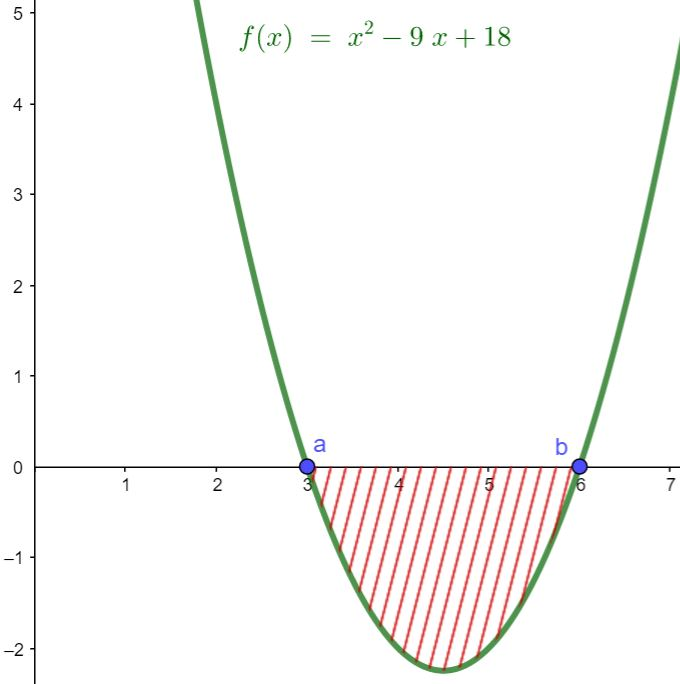
\includegraphics[width=\linewidth]{sol55}\end{figure}\end{minipage}
\end{minipage}
$F(x) = \frac13x^3 - \frac92x^2 + 18x + C$. Получаем, что $S = F(6) - F(3) = \frac13\cdot(6^3 - 3^3) - \frac92\cdot(6^2 - 3^2) + 18\cdot(6 - 3) + C - C = \frac{216 - 27}{3} - \frac{9\cdot27}{2} + 18\cdot3 = 63 - 121{,}5 + 54 = -4{,}5$.\\
Площадь получилась отрицательной, потому что вся находится в отрицательной области, абсолютная величина же равна $4{,}5$.}
{Площадь фигуры (абсолютная величина) равна $4{,}5$.}{Применить формулу $S = F(b) - F(a)$, предварительно найдя точки пересечения $b$ и $a$. Подумать о том, какой должен быть знак.}
\end{problem}

\begin{problem}{Вычисление площадей.}{11.3.5}{10A}{(лёгкая)}
{Найти площадь плоской фигуры, которая ограничена координатными прямыми, прямой $x = 1$, и функцией $y(x) = -e^{x}$.}
{\vspace{-6mm}\\\begin{minipage}{\linewidth}
    \begin{minipage}{0.58\linewidth}
    ~\vspace{5mm}\\
    Одна из координатных прямых~--- $x = 0$, поэтому наша фигура находится между $x = 0$ и $x = 1$. Сверху она ограничена осью абсцисс, снизу экспонентой.\smallskip\\ То есть нам нужно найти площадь фигуры, изображённой на рисунке справа.\smallskip\\
    По теореме Ньютона-Лейбница площадь фигуры в данном случае может быть вычислена по формуле $S = F(b) - F(a)$.\smallskip\\
    Находим первообразную: $F(x) = -e^x + C$.\\ Получаем, что $S = F(1) - F(0) = -e^1 - (-e^0) + C - C = -e + 1 = 1 - e \approx -1{,}718$.\smallskip\\ Площадь получилась отрицательной, потому что она вся находится в отрицательной области, абсолютная величина же равна $e - 1 \approx 1{,}718$.
    \end{minipage}
    \hspace{0.05\linewidth}
    \begin{minipage}{0.36\linewidth}\begin{figure}[H] 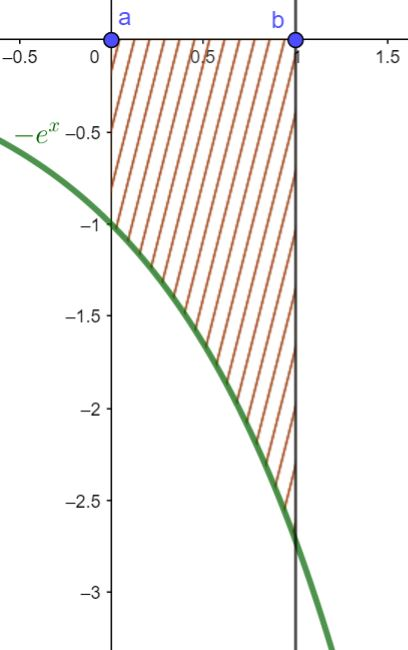
\includegraphics[width=\linewidth]{sol56}\end{figure}\end{minipage}
\end{minipage}}
{$S = e - 1 \approx 1{,}718$.}{Применить формулу $S = F(b) - F(a)$, выяснив чему равны $b$ и $a$. Подумать о том, какой должен быть знак у площади.}
\end{problem}

\begin{problem}{Вычисление площадей.}{11.3.5}{10A}{(лёгкая)}
{Найти площадь фигуры, ограниченной линиями $y = x + 1$, $\,y = \frac2x$, $y = 0$, $x = 3$ (сначала аккуратно нарисовать все графики на координатной плоскости).}
{Выясним, что с чем пересекается: $y = x + 1$ пересекается с $y = \frac{2}{x}$ $\;\Rightarrow\; x + 1 = \frac2x \;\Rightarrow\; x^2 + x - 2 = 0 \;\Rightarrow\; x = 1; \, x = -2$.\\ Точки пересечения прямой и гиперболы~--- $(1; 2)$ и $(-2; -1)$.\\ Прямая $y = x + 1$ пересекается с $y = 0$ в $x = -1$, точка пересечения $(-1; 0)$.\\
Точки пересечения прямой $x = 3$ с осью абсцисс и гиперболой~--- $(3; 0)$ и $(3; \frac23)$. \vspace{-4mm}\\\begin{minipage}{\linewidth}
    \begin{minipage}{0.55\linewidth}
    ~\vspace{1mm}\\
    Таким образом, интересующая нас фигура выглядит так, как показано на рисунке справа, координаты всех указанных точек мы уже нашли.\smallskip\\ Чтобы найти площадь под графиком, нужно вычислить определённый интеграл.
    \end{minipage}
    \hspace{0.01\linewidth}
    \begin{minipage}{0.43\linewidth}\begin{figure}[H] 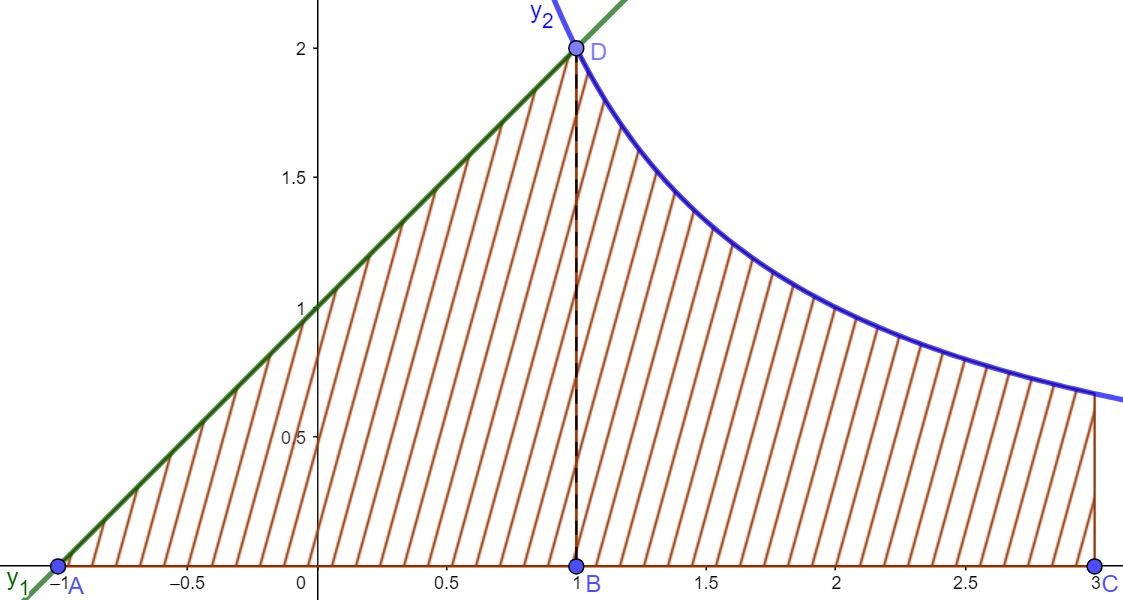
\includegraphics[width=\linewidth]{sol62}\end{figure}\end{minipage}\smallskip
\end{minipage}
В данном случае можно использовать аддитивность интеграла: искомая площадь равна сумме двух площадей, и $S = \int\limits_{-1}^1 (x+1)\, dx + \int\limits_1^3 \frac2x \,dx = \left.\left(\frac{x^2}{2} + x\right)\right|_{-1}^1 + \left.2\ln x\vphantom{\frac11}\right|_1^3 = $ $= \frac12 + 1 - \frac{(-1)^2}{2} - (-1) + 2\ln 3 - 2\ln 1 = 2 + 2\ln 3 = 2(1 + \ln 3)$.}
{Площадь указанной фигуры равна $2(1 + \ln 3) \approx 4{,}197$.}{Разбей площадь данной фигуры на две более простых площади.}
\end{problem}

\begin{problem}{Вычисление площадей.}{11.3.5}{10A}{*}
{Найти площадь фигуры, ограниченной линиями $y_1(x) = -x$, $\,y_2(x) = 2x - x^{2}$ (сначала нарисовать на координатной плоскости параболу и прямую и понять, каковы пределы интегрирования).}
{\vspace{-3mm}\\\begin{minipage}{\linewidth}
    \begin{minipage}{0.59\linewidth}
    ~\vspace{2mm}\\
    Изобразим графики функций $y_1(x) = -x$ и $y_2(x) = 2x - x^2$: получается, что фигура имеет вид, изображённый на рисунке справа. Найдём точки пересечения прямой и параболы (графические методы не позволяют ничего посчитать): $-x = 2x - x^2 \;\Rightarrow\; 3x - x^2 = 0 \;\Rightarrow\; x(3 - x) = 0$.\smallskip\\ Значит, парабола и прямая пересекаются в точках $A (0; 0)$ и $B (3; -3)$. То есть для нахождения площади нужно найти определённый интеграл от 0 до 3 от какой-то функции.\\ Разберёмся, что это за функция: суммируются величины $f(x)$, при $x$, меняющемся от 0 до 3.
    \end{minipage}
    \hspace{0.05\linewidth}
    \begin{minipage}{0.35\linewidth}\begin{figure}[H] 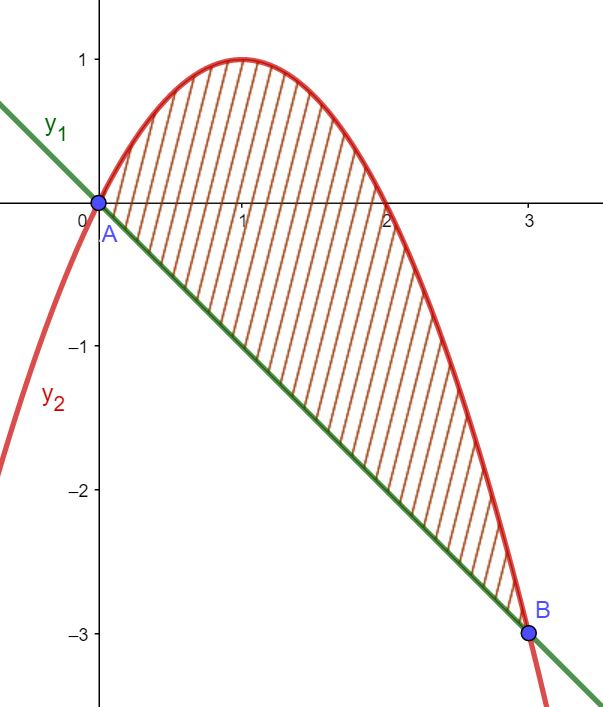
\includegraphics[width=\linewidth]{sol57}\end{figure}\end{minipage}
\end{minipage}
\smallskip\\После размышлений можно понять, что интеграл берётся от функции $y_2(x) - y_1(x)$: везде на этом отрезке $y_2(x) \geqslant y_1(x)$ и $y_2(x) - y_1(x)$ является длиной вертикального отрезка, рассекающего эту фигуру по точкам с абсциссой $x$.\\ Вычисляем определённый интеграл: $\int\limits_0^3 ((2x - x^2) - (-x)) \, dx = \int\limits_0^3 (3x - x^2) \, dx = $ $\left.(\frac32x^2 - \frac13x^3)\right|_{0}^3 = \frac32\cdot9 - \frac13\cdot 3^3 = 13{,}5 - 9 = 4{,}5$.\\ Таким образом, площадь образующейся фигуры равна $4{,}5$.}
{Площадь фигуры, которая ограничена линиями $y_1(x) = -x$ и $y_2(x) = 2x - x^2$, равна $4{,}5$.}{Интегрироваться будет функция $f(x) = y_2(x) - y_1(x)$. Почему?}
\end{problem}

\begin{problem}{Вычисление площадей.}{11.3.5}{10A}{*}
{Найти площадь фигуры, ограниченной линиями $y_1(x) = x^2 - 2$, $\,y_2(x) = 2x + 1$ (сначала нарисовать на координатной плоскости параболу и прямую и понять, каковы пределы интегрирования).}
{\vspace{-4mm}\\\begin{minipage}{\linewidth}
    \begin{minipage}{0.59\linewidth}
    ~\vspace{1mm}\\
    Выясним, где пересекаются эти прямая и парабола: $y_1(x) = y_2(x) \;\Rightarrow\; x^2 - 2 = 2x + 1 \;\Rightarrow\; x^2 - 2x - 3 = 0 \;\Rightarrow\; x = 3;\, x = -1$.\smallskip\\ Поэтому фигура имеет вид, изображённый на рисунке справа. Чтобы найти данную площадь, нужно вычислить определённый интеграл.\smallskip\\
    А так как $y_2(x) - y_1(x)$ равно высоте данной фигуры в точке $x$, площадь этой фигуры по определению интеграла равна $\int\limits_{-1}^3 (y_2(x) - y_1(x))\, dx =$
    $= \int\limits_{-1}^3 (2x + 1 - (x^2 - 2))\, dx = \int\limits_{-1}^3 (3 + 2x - x^2)\, dx$.
    $\int\limits_{-1}^3 (3 + 2x - x^2)\, dx = \left.\left(3x + x^2 - \frac{x^3}{3}\right)\right|_{-1}^3 = 9 + 9 - \frac{27}{3} - \left(-3 + (-1)^2 - \frac{(-1)^3}{3}\right) = 11 - \frac13 = 10\frac23$.
    \end{minipage}
    \hspace{0.04\linewidth}
    \begin{minipage}{0.36\linewidth}\begin{figure}[H] 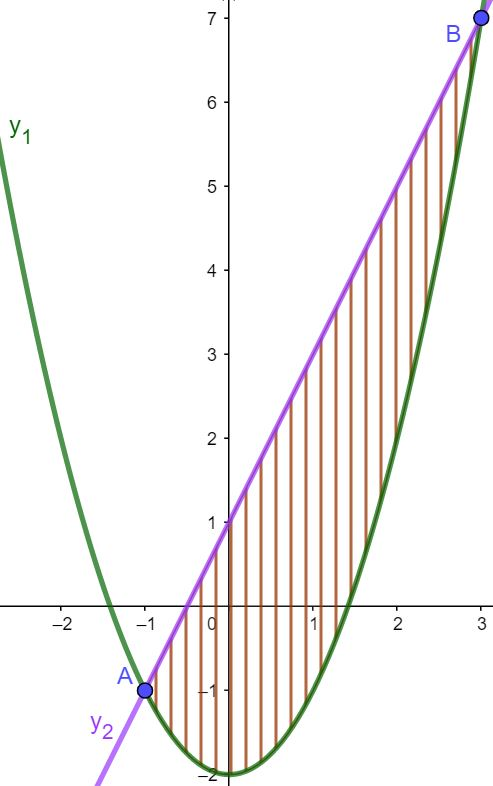
\includegraphics[width=\linewidth]{sol63}\end{figure}\end{minipage}\smallskip
\end{minipage}}
{Площадь данной фигуры равна $10\frac23$.}{Площадь криволинейной трапеции, заключённой между функциями $f(x)$ и $g(x)$, может быть вычислена как $\int\limits_a^b (f(x) - g(x)) \, dx$, если $f > g$ на $[a; b]$.}
\end{problem}

\begin{problem}{Вычисление площадей.}{11.3.5}{10A}{*}
{Найти площадь фигуры, ограниченной линиями $y_1(x) = x^2 + x$, $\,y_2(x) = 1 - x^2$ (сначала нарисовать на координатной плоскости параболы и понять, каковы пределы интегрирования).}
{Выясним, в каких точках эти параболы пересекаются: $y_1(x) = y_2(x) \;\Rightarrow\; x^2 + x = 1 - x^2 \;\Rightarrow\; 2x^2 + x - 1 = 0 \;\Rightarrow\; D = 9 \;\Rightarrow\; x = -1;\, x = \frac12$.\smallskip\\\vspace{-4mm}\\\begin{minipage}{\linewidth}
    \begin{minipage}{0.59\linewidth}
    ~\vspace{1mm}\\
    Поэтому фигура имеет вид, изображённый на рисунке справа. Чтобы найти данную площадь, нужно вычислить определённый интеграл.\smallskip\\
    $y_2(x) - y_1(x)$ равно высоте этой фигуры в точке $x$, поэтому площадь этой фигуры по определению интеграла равна $\int\limits_{-1}^{\frac12} (y_2(x) - y_1(x))\, dx$.
    \end{minipage}
    \hspace{0.04\linewidth}
    \begin{minipage}{0.36\linewidth}\begin{figure}[H] 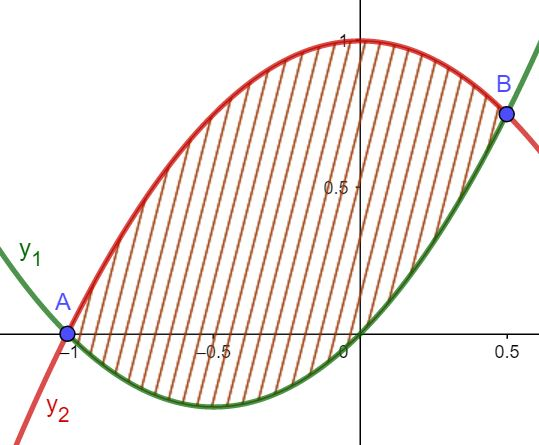
\includegraphics[width=\linewidth]{sol64}\end{figure}\end{minipage}\smallskip
\end{minipage}
$\int\limits_{-1}^{\frac12} (y_2(x) - y_1(x))\, dx = \int\limits_{-1}^{\frac12} (1 - x^2 - (x^2 + x))\, dx = \int\limits_{-1}^{\frac12} (1 - x - 2x^2)\, dx = \left.\left(x - \frac{x^2}{2} - \frac{2x^3}{3}\right)\right|_{-1}^{\frac12} = \frac12 - \frac18 - \frac{1}{12} - \left(-1 - \frac12 - \frac{2\cdot(-1)^3}{3}\right) = 2 - \frac18 - \frac{1}{12} - \frac23 = 1\frac18 = 1{,}125$.}
{Площадь указанной фигуры составляет $1{,}125$.}{Площадь криволинейной трапеции, заключённой между функциями $f(x)$ и $g(x)$, может быть вычислена как $\int\limits_a^b (f(x) - g(x)) \, dx$, если $f > g$ на $[a; b]$.}
\end{problem}

\begin{problem}{Вычисление площадей.}{11.3.5}{10A}{*}
{Найти площадь фигуры, ограниченной линиями $x + y = 4$, $\,xy = 3$ (сначала нарисовать графики на координатной плоскости).}
{Перепишем уравнения, задающие наши линии, выразив $y$:\\
$x + y = 4 \;\Rightarrow\; y = 4 - x$. $\;xy = 3 \;\Rightarrow\; y = \frac3x$.
\vspace{-5mm}\\\begin{minipage}{\linewidth}
    \begin{minipage}{0.59\linewidth}
    ~\vspace{2mm}\\
    Выясним, где данные линии пересекаются:\\ $4 - x = \frac3x \;\Rightarrow\; 4x - x^2 - 3 = 0 \;\Rightarrow\; x = 1; \,x = 3$.\medskip\\
    Следовательно, поскольку везде на отрезке $[1; \,3]$ прямая лежит выше гиперболы ($4 - x > \frac3x$), площадь фигуры $S$ может быть найдена c помощью следующего определённого интеграла:\vspace{-3mm} $$S = \int\limits_1^3 \left(4 - x - \frac3x\right) \, dx.$$
    \vspace{-4mm}\\
    $\int\limits_1^3 (4 - x - \frac3x) \, dx = \left.\left(4x - \frac{x^2}{2} - 3\ln x\right)\right|_{1}^{3} = 12 - 4{,}5 - 3\ln 3 - (4 - 0{,}5 - 3\ln 1) = 4 - 3\ln 3$.
    \end{minipage}
    \hspace{0.04\linewidth}
    \begin{minipage}{0.36\linewidth}\begin{figure}[H] 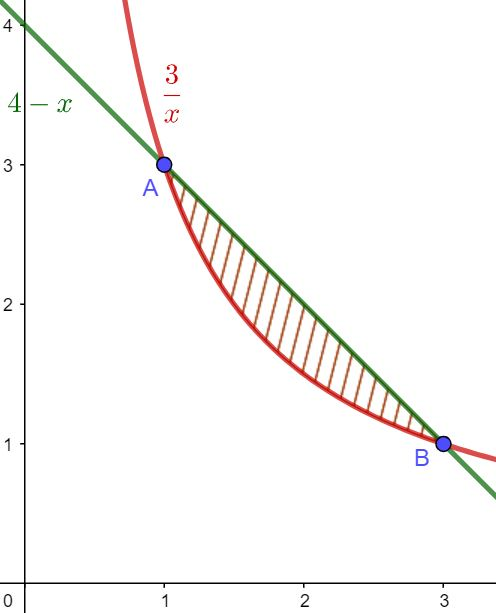
\includegraphics[width=\linewidth]{sol65}\end{figure}\end{minipage}\smallskip
\end{minipage} }
{Площадь данной фигуры равна $4 - 3\ln 3 \approx 0{,}704$.}{Площадь криволинейной трапеции, заключённой между функциями $f(x)$ и $g(x)$, может быть вычислена как $\int\limits_a^b (f(x) - g(x)) \, dx$, если $f > g$ на $[a; b]$.}
\end{problem}

\begin{problem}{Вычисление площадей.}{11.3.5}{10A}{*}
{Найти площадь фигуры, ограниченной линиями $y = x^3 - x + 1$, $\,y = -\frac78$, $x = \frac12$ (сначала аккуратно нарисовать график на координатной плоскости).}
{Выясним, в каких точках происходят пересечения: есть пересечение перпендикулярных прямых в точке $B = (\frac12;\, -\frac78)$, есть точка $C = (\frac12;\, \frac58)$. 
\smallskip\\\vspace{-4mm}\\\begin{minipage}{\linewidth}
    \begin{minipage}{0.61\linewidth}
    ~\vspace{1mm}\\
    Найдём точку пересечения $y = x^3 - x + 1$ и $y = -\frac78$:\smallskip\\ $\;x^3 - x + 1 = - \frac78 \;\Rightarrow \; x^3 - x + \frac{15}{8} = 0 \;\Rightarrow\; (x + \frac32)\cdot(x^2 - \frac32x + \frac54) = 0 \;\Rightarrow\; x = -\frac32\,$. \\(поскольку для квадратного $D = \frac94 - 4\cdot\frac54 < 0$).\medskip\\
    То есть $A = (-\frac32;\, -\frac78)$. Следовательно, фигура имеет вид, изображённый на рисунке справа: \medskip\\
    Высота этой фигуры в точке $x$ равна $x^3 - x + \frac{15}{8}$,\\ поэтому площадь этой фигуры по определению интеграла равна $S = \int\limits_{-\frac32}^{\frac12} (x^3 - x + \frac{15}{8})\, dx$.
    \end{minipage}
    \hspace{0.02\linewidth}
    \begin{minipage}{0.36\linewidth}\begin{figure}[H] 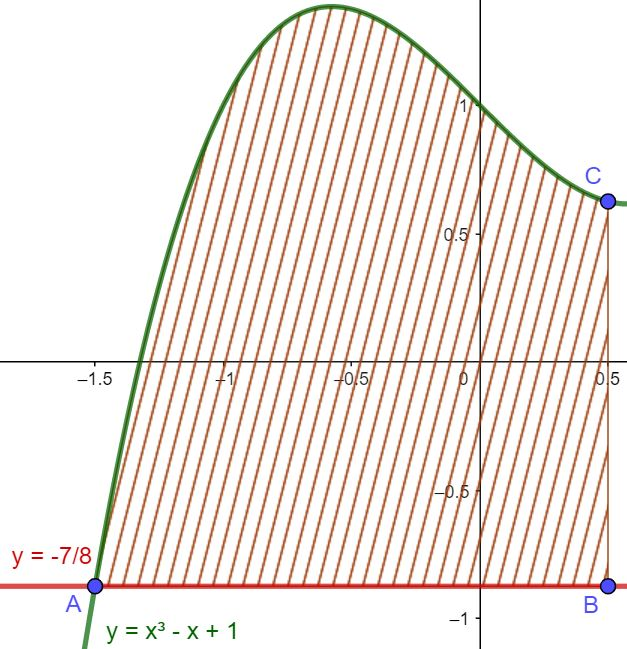
\includegraphics[width=\linewidth]{sol66}\end{figure}\end{minipage}\smallskip
\end{minipage}
$\int\limits_{-\frac32}^{\frac12} (x^3 - x + \frac{15}{8})\, dx = \left.\left(\frac{x^4}{4} - \frac{x^2}{2} + \frac{15}{8}x\right)\right|_{-\frac32}^{\frac12} = \frac{1}{64} - \frac18 + \frac{15}{16} - \left(\frac{81}{64} - \frac{9}{8} - \frac{45}{16}\right) = -\frac{80}{64} + 1 + \frac{60}{16} = -\frac54 + 1 + \frac{15}{4} = 3{,}5$.}
{Площадь указанной фигуры составляет $3{,}5$.}{Площадь криволинейной трапеции, заключённой между функциями $f(x)$ и $g(x)$, может быть вычислена как $\int\limits_a^b (f(x) - g(x)) \, dx$, если $f > g$ на $[a; b]$.}
\end{problem}

\begin{problem}{Вычисление площадей.}{11.3.5}{10A}{*}
{Интеграл $I(a) = \displaystyle\int_{a-1}^{a+1} \!\!f(x) \, dx$ равен площади под графиком функции $f(x)$ на отрезке $[a\!-\!1;\, a\!+\!1]$. Найти, при каком вещественном $a$ эта площадь будет наименьшей из всех возможных, если $f(x) = x^2 - 5x + 7$.}
{\vspace{-6mm}\\\begin{minipage}{\linewidth}
    \begin{minipage}{0.58\linewidth}
    Квадратный трёхчлен $x^2 - 5x + 7$ имеет отрицательный дискриминант $D = 25 - 28 < 0$ и положительный старший коэффициент, поэтому данная парабола находится выше оси абсцисс и любой определённый интеграл будет положителен. Поскольку пределы интегрирования --- $a-1$ и $a+1$, в каждом случае получается <<окно>> шириной 2. Пусть $a$ --- какое-то неизвестное нам число, вычислим определённый интеграл:\\
    $\int \!f(x) \,dx = \frac{1}{3}x^3 - \frac52x^2 + 7x + C \;\Rightarrow\;$ \\$\displaystyle\int_{a-1}^{a+1} \!\!(x^2 - 5x + 7) \, dx = \left(\frac{1}{3}x^3 - \frac52x^2 + 7x\right|_{a-1}^{a+1} =$ $= \frac13((a+1)^3 - (a-1)^3) - \frac52 ((a+1)^2 - (a-1)^2) + 7(a+1 - (a - 1)) = \frac13(6a^2 + 2) - 10a + 14 = $ $= 2f(a) + \frac23$.
    \end{minipage}
    \hspace{0.01\linewidth}
    \begin{minipage}{0.35\linewidth}\begin{figure}[H] 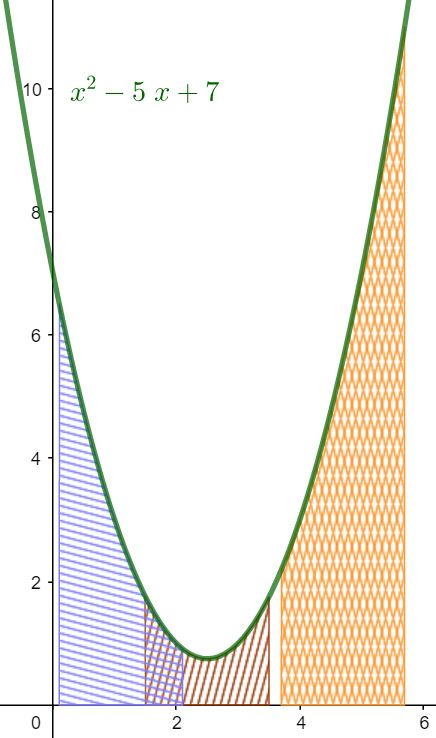
\includegraphics[width=\linewidth]{sol68}\end{figure}\end{minipage}
\end{minipage}
Итого, $I(a) = 2f(a) + \frac23$. Для нахождения минимума $I(a)$ находим производную: $I'(a) = 2\cdot(2a - 5)$. $\;I'(a) = 0 \;\Rightarrow\; a = 2{,}5$ (вершина параболы).}
{Данная площадь $S = I(a)$ будет наименьшей, если взять $a = 2{,}5$.\\ Площадь в этом случае будет равна $2f(2{,}5) + \frac23 = \frac32 + \frac23 = \frac{13}{6} \approx 2{,}17$.}{Вычисли определённый интеграл (он будет зависеть от $a$), а затем с помощью производной найди минимум этого выражения.}
\end{problem}

\begin{problem}{Вычисление площадей.}{11.3.5}{10A}{*}
{Интеграл $\displaystyle\int_{b-1}^{b+1} \!\!e^{-|x|} \, dx$  равен площади под графиком функции $f(x) = e^{-|x|}$ на отрезке $[b\!-\!1;\, b\!+\!1]$. Нарисовать график этой функции и выяснить, при каком вещественном $b$ эта площадь будет максимальна.}
{Для того, чтобы правильно раскрыть модуль во всех случаях, будем действовать аккуратно. Во-первых, подынтегральная функция $f(x) = e^{-|x|}$ равна $e^x$ при $x \leqslant 0$ и равна $e^{-x}$ при $x \geqslant 0$. Далее, для нахождения интеграла нам понадобится первообразная функции $f(x)$. При $x \leqslant 0$ первообразной $f_1(x) = e^x$ является $e^x + C$, при $x \geqslant 0$, первообразной для $f_2(x) = e^{-x}$ будет $-e^{-x} + C$.\\
Согласно формуле Ньютона-Лейбница, $I(b) = \displaystyle\int_{b-1}^{b+1} \!\!f(x) \, dx = F(b + 1) - F(b - 1)$.\\
Рассмотрим отдельно три случая:\medskip\\ \textbf{1)} $b - 1 < b + 1 \leqslant 0$. Тогда $F(x) = e^x$, и интеграл равен $e^{b+1} - e^{b-1} = e^b\cdot(e - \frac1e)$.\\ В этом случае $b \leqslant -1$, а при поиске максимума мы получаем, что $e^b$ должно быть как можно больше (ведь $e - \frac1e > 0$, $e^b$ --- монотонно возрастающая). То есть $b = -1$.\smallskip\\
\textbf{2)} $0 \leqslant b - 1 < b + 1$, или $b \geqslant 1$. Тогда $F(x) = -e^{-x}$, $I(b) = -e^{-(b+1)}-(-e^{-(b-1)}) = e^{-b}\cdot(e - \frac1e)$. При поиске максимума, так как $e - \frac1e > 0$, а $e^{-x}$ --- монотонно убывающая функция, получаем, что $b$ должно быть как можно меньше, то есть $b = 1$.\smallskip\\
\textbf{3)} Случай, когда левый предел интегрирования неположителен, а правый --- неотрицателен: $b - 1 \leqslant 0 \leqslant b + 1$. В этом случае $I(b) = -e^{-(b+1)} - e^{b-1} = -\frac1e\cdot(e^b + e^{-b})$.\\
Мы ищем максимум этого выражения, причём только для $b \in [-1;\, 1]$.\\ $I'(b) = -\frac1e\cdot(e^b - e^{-b})$. Находим критическую точку: $I'(b) = 0 \;\Rightarrow\; e^b - e^{-b} = 0 \;\Rightarrow\; e^b = e^{-b} \;\Rightarrow\; b = -b \;\Rightarrow\; b = 0$. Несложно убедиться, что это действительно точка максимума (левее производная положительна, правее --- отрицательна).\smallskip\\
Таким образом, все значения $b$, такие что $|b| > 1$, проигрывают $b = \pm 1$, а те, в свою очередь, проигрывают $b = 0$ (смотри на график функции $f(x)$ ниже)
\vspace{-4mm}\\\begin{minipage}{\linewidth}
    \begin{figure}[H] 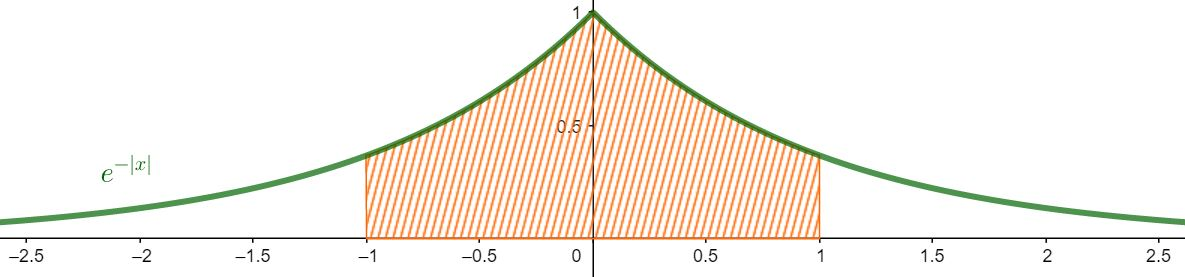
\includegraphics[width=\linewidth]{sol69}\end{figure}
\end{minipage}
\vspace{-1mm}
$$I(0) = \int_{-1}^0 \!e^x \,dx + \int_0^1 \!e^{-x} \,dx = e^0 - e^{-1} + (-e^{-1}) - (-e^0) = 2 - \frac2e \approx 1{,}26.$$}
{Площадь будет максимальна при $b = 0$. $\;S_{\text{max}} = I(0) = 2 - \frac2e \approx 1{,}26$.}{Вычисли определённый интеграл (он будет зависеть от $b$), а затем с помощью производной найди максимум этого выражения.\\
Для того, чтобы аккуратно избавиться от модуля, надо рассмотреть три случая: \textbf{1) } $b - 1 < b + 1 \leqslant 0,\qquad\qquad$ \textbf{2) } $0 \leqslant b - 1 < b + 1,\qquad\qquad$ \textbf{3) } $b - 1 \leqslant 0 \leqslant b + 1$.}
\end{problem}

\begin{problem}{Вывод некоторых формул с помощью интегрирования.}{11.3.6}{10A}{(лёгкая)}
{Представим конус с радиусом $r$ и высотой $h$. Если на его высоте разместить на равных расстояниях друг от друга $n + 1$ точку, то высота разделится на $n$ равных отрезков. Проведём через них плоскости, перпендикулярные высоте. Пусть $r(x)$~--- радиус окружности сечения, получающейся в результате сечения конуса одной из упомянутых выше плоскостей, проходящей через точку на высоте $x$.\\ Рассмотрим суммы $V_n = \sum\limits_{k = 1}^{n} \pi r^2\!\left(k\cdot\frac{h}{n}\right)\cdot\frac{h}{n}$. Объяснить, почему $\lim\limits_{n\to\infty} V_n = V_{\text{конуса}}$.\\
Найти функцию $r(x)$, показывающую радиус сечения на высоте $x$ от основания конуса. Получить формулу для объёма конуса, вычислив определённый интеграл ~\hspace*{5cm}$V_{\text{конуса}} = \displaystyle \int\limits_{0}^{h} \pi \cdot \left(r\cdot\frac{h - x}{h}\right)^2 \,dx$.}
{НаписанноеРешение}
{ВерныйОтвет}{Подсказка}
\end{problem}

\begin{problem}{Вывод некоторых формул с помощью интегрирования.}{11.3.6}{10A red переписать на треугольную пирамиду и обобщение}{*}
{Представим произвольную пирамиду, площадь основания которой равна $S$, а высота равна $h$. Если на её высоте разместить на равных расстояниях друг от друга $n + 1$ точку, то высота разделится на $n$ равных отрезков. Проведём через них плоскости, перпендикулярные высоте. Пусть $S(x)$~--- площадь сечения, получающегося в результате сечения пирамиды одной из упомянутых выше плоскостей, проходящей через точку на высоте $x$.\\ Рассмотрим суммы $V_n = \sum\limits_{k = 1}^{n} S\!\left(k\cdot\frac{h}{n}\right)\cdot\frac{h}{n}$. Объяснить, почему $\lim\limits_{n\to\infty} V_n = V_{\text{пирамиды}}$.\\
Обосновать, почему $S(x) = S\cdot\left(\frac{h - x}{h}\right)^2$, и получить формулу для объёма произвольной пирамиды, вычислив соответствующий определённый интеграл.}
{Разберёмся со всем по порядку. Зафиксируем $n$. Тогда после того, как на высоте отметили $n + 1$ точку, получаем точку в основании, точку на высоте $\frac hn$, точку на высоте $\frac{2h}{n}$, ... точку на высоте $h$. Теперь рассмотрим нашу сумму $V_n = \sum\limits_{k = 1}^{n} S\!\left(k\cdot\frac{h}{n}\right)\cdot\frac{h}{n}$. Что из себя представляет какое-нибудь одно слагаемое?\\ Посмотрим: $S\!\left(k\cdot\frac{h}{n}\right)\cdot\frac{h}{n}$~--- произведение площади сечения, проходящего через точку на высоте $\frac{kh}{n}$, на длину $\frac{h}{n}$. Так как $k$ меняется от 1 до $n$, первая же точка находится на высоте $\frac{h}{n}$ над основанием, и $\frac{h}{n}$ задаёт высоту прямой призмы с основанием $S\!\left(\frac{h}{n}\right)$ (которая находится внутри нашей пирамиды).\\ Аналогично для всех остальных $k$: то есть каждое слагаемое~--- это объём призмы с основанием $S\!\left(k\cdot\frac{h}{n}\right)$, зажатой на высоте $H \in \left[\frac{(k - 1)h}{n};\, \frac{kh}{n}\right]$.\\ Понятно, что сумма объёмов всех этих прямых призм $V_n$ меньше объёма пирамиды, поскольку все эти призмы полностью содержатся в ней. Однако, при $n \to +\infty$, получающихся слоёв-призм становится всё больше, и получающаяся <<башенка>> всё точнее и точнее приближает пирамиду. А значит, $\lim\limits_{n\to+\infty} V_n = V_{\text{пирамиды}}$.\smallskip\\
Приведу краткое доказательство равенства $S(x) = S\cdot\left(\frac{h - x}{h}\right)^2$ для треугольной пирамиды (поскольку любую другую пирамиду можно разрезать на несколько треугольных). Если в основании у пирамиды треугольное основание $ABC$, то сечение на высоте $x$ (на расстоянии $h - x$ от вершины) будет подобным треугольником $A_1B_1C_1$ (в силу того, что $AB \parallel A_1B_1$, $BC \parallel B_1C_1$, $AC \parallel A_1C_1$, у треугольников равны все углы). Коэффициент подобия $k$ равен отношению $\frac{h - x}{h}$.\\ Поэтому площадь изменяется в $k^2$ раз, то есть $S(x) = S\cdot\left(\frac{h - x}{h}\right)^2$.\smallskip\\
Значит, $V_{\text{пирамиды}} = \int\limits_0^h S(x)\,dx = \int\limits_0^h S\cdot\left(\frac{h - x}{h}\right)^2 dx = \frac{S}{h^2}\cdot \int\limits_0^h (h^2 - 2hx + x^2)\,dx = $\\
$\frac{S}{h^2}\cdot\left.\left(h^2 x - hx^2 + \frac13x^3\right)\right|_0^h = \frac{S}{h^2}\cdot\left(h^3 - h^3 + \frac13h^3 - 0 + 0 - 0\right) = \frac{S}{h^2}\cdot\frac13h^3 = \frac13 Sh$.}
{Объём пирамиды может быть найден с помощью определённого интеграла и составляет одну треть от произведения площади основания на высоту: \vspace{-3mm} $$V_{\text{пирамиды}} = \tfrac13 Sh.$$ \vspace{-6mm}}{Каждое слагаемое этой суммы~--- объём некоторой призмы.\\ В конце достаточно рассмотреть треугольную пирамиду.
$\;V_{\text{пирамиды}} = \int\limits_0^h S(x)\,dx$.}
\end{problem}

\begin{problem}{Вывод некоторых формул с помощью интегрирования.}{11.3.6}{10A red}{*}
{Представим шар радиуса $r$. Мысленно разрежем его на два равных полушария и положим плоской частью на некоторую плоскость $\alpha$. Будем проводить сечения, параллельные плоскости $\alpha$. Пусть $S(x)$, $x \in[0, r]$~--- площадь окружности, получающейся в результате сечения полушария такой плоскостью, которая находится на высоте $x$ над плоскостью $\alpha\,$ ($S(0) = \pi r^2$, $\,S(r) = 0$).\smallskip\\ 
1) Показать, что $S(x) = \pi(r^2 - x^2)$.\smallskip\\
2) Использовать последовательность интегральных сумм $V_n$, которая сходится к $V_{\text{полушария}}$, составить определённый интеграл $\int\limits_{A}^{B} f(x) \,dx = V_{\text{полушария}}$, вычислить его как функцию от $r$ и получить таким образом формулу для объёма шара.}
{Что происходит, если провести сечение на высоте $x$? Пусть $O$~--- центр шара, $H$~--- центр получающегося круга (и $OH = x$), $K$~--- точка на границе этого круга. Обозначим $KH = R$. Тогда, во-первых, $OK = r$ (точка на границе шара), а во-вторых, $\triangle KOH$~--- прямоугольный, $\angle KHO = 90^\circ$. Следовательно, по теореме Пифагора, $KH^2 + OH^2 = OK^2$, откуда $R^2 + x^2 = r^2$, откуда $R^2 = r^2 - x^2$.\\
То есть полученная при сечении окружность имеет радиус $R = \sqrt{r^2 - x^2}$, а значит, площадь сечения $S(x) = \pi(r^2 - x^2)$.\smallskip\\
Теперь разбираемся с интегральными суммами. Если рассмотреть сумму вида $V_n = \sum\limits_{k = 1}^{n} S\!\left(k\cdot\frac{r}{n}\right)\cdot\frac{r}{n}$, то данная сумма представляет собой сумму объёмов $n$ цилиндров одинаковой высоты $\frac{r}{n}$, которые все лежат внутри полушария и касаются его границы. И поскольку с увеличением числа цилиндров, получаемая башенка по очертаниям всё ближе приближается к нашему полушарию, с увеличением $n$ мы получим более точное приближение, и в пределе $\lim\limits_{n\to+\infty} V_n = V_{\text{полушария}}$.\\
Это означает, что $V_{\text{полушария}} = \int\limits_0^r S(x) \,dx = \int\limits_0^r \pi(r^2 - x^2) \,dx = \pi\cdot\int\limits_0^r (r^2 - x^2) \,dx = $\\
$\pi\cdot\left.\left(r^2x - \frac13x^3\right)\right|_0^r = \pi\cdot(r^3 - \frac13r^3 - 0 + 0) = \pi\cdot\frac23r^3 = \frac23\pi r^3$.\smallskip\\
Итого, $V_{\text{полушария}} = \frac23\pi r^3$, а объём шара вдвое больше и равен $V_{\text{шара}} = \frac43\pi r^3$.}
{Объём шара радиуса $r$ равен объёму двух полушарий и составляет \vspace{-3mm} $$V_{\text{шара}} = \frac43\pi r^3.$$ \vspace{-6mm}}{Каждое слагаемое в искомой последовательности интегральных сумм~--- объём некоторого цилиндра, причём вместе эти цилиндры должны хорошо приближать объём полушария. Итоговый объём надо не забыть удвоить.}
\end{problem}

\begin{problem}{Вывод некоторых формул с помощью интегрирования.}{11.3.6}{10A}{(лёгкая)}
{Считая, что Земля~--- идеальный шар с радиусом 6370 км, оценить её среднюю плотность, если известно, что масса Земли составляет $5{,}97\cdot10^{24}$ кг.}
{Предположив, что Земля --- идеальный шар, мы можем вычислить её объём: $V_{\text{земли}} = \frac43 \pi r^3$. Плотность равна отношению массы к объёму:\\ $\displaystyle\rho_{\text{ср}} = \frac{m_{\text{земли}}}{V_{\text{земли}}} = \frac{3m_{\text{земли}}}{4\pi r^3} = \frac{3\cdot5{,}97\cdot10^{24}}{4\pi\cdot(6370\cdot10^3)^3} \text{кг/м}^3 = \frac{3\cdot5{,}97\cdot10^6}{4\pi\cdot6{,}37^3}\text{кг/м}^3 \approx 5514\text{кг/м}^3$.}
{Средняя плотность Земли составляет 5500 кг/м$^3$, или $5{,}5$ г/см$^3$.}{Использовать формулу для объёма шара.}
\end{problem}

\begin{problem}{Вывод некоторых формул с помощью интегрирования.}{11.3.6}{10A}{(лёгкая)}
{Радиусы трёх сплошных металлических шариков равны 3, 4 и 5 см соответственно. Эти шарики расплавили, и из получившегося металла отлили новый сплошной шар. Чему будет равен его радиус?}
{НаписанноеРешение}
{ВерныйОтвет}{Подсказка}
\end{problem}

\end{document}